% Week 10: curvature shapes (FPCA) in the proximal and mid LAD. Input from week10.tex.
\subsection*{Curvature shapes in the proximal and mid LAD}
In the main model, curvature enters as the mean turning $T_5$ of each of the nine segments. Taking the mean per segment rather than per artery or per person
already keeps part of the position: a bend in the proximal LAD and a bend in the distal LAD enter the
model as different variables. Within a segment, however, the position of the bends is averaged away,
and much information may still be lost: a segment with one sharp bend and a segment that turns gently
along its whole length can have the same mean. I therefore want a descriptive analysis of whether the
position of the bends within a segment matters beyond the mean turning. My solution is to use FPCA to find the main shapes of the turning profile along each segment, and then test whether the scores along those shapes add to the mean turning in predicting plaque development.


I can only do the descriptive analysis in the proximal and mid LAD, as these are the only segments with enough events to estimate the association of \textbf{several} curvature shapes with incident plaque: 275 and 201 of the
1{,}077 plaque-free participants developed plaque there, which by the Riley criteria allows 10 and 8
terms at an anticipated C of 0.70, against at most 5 in the other segments. 

\textbf{Turning profile.} I compute the turning angle at every
centerline point 5\,mm apart: the angle between the 5\,mm chord arriving at the
point and the 5\,mm chord leaving it, divided by $\ell = 5$\,mm, which gives $\kappa$ in rad/mm
(Figure~\ref{fig:sliding}). The profile is then cut at the segment boundaries. Segment length and point spacing differ between
people, so to compare profiles position by position, each is linearly interpolated onto 50 equally
spaced positions of normalised segment length (0 at the start, 1 at the end of the segment). A position thus refers to the same relative
place in every person: position 25 lies halfway along the segment, whether the segment is 30 or
50\,mm long. Each
segment thus gives an $n \times 50$ matrix $M$, where $M_{ij}$ is the turning of person $i$ at
position $j$. No further smoothing is applied, as the profile has a value at every centerline point
and the tracer already smooths the points.

\begin{figure}[h]
  \centering
  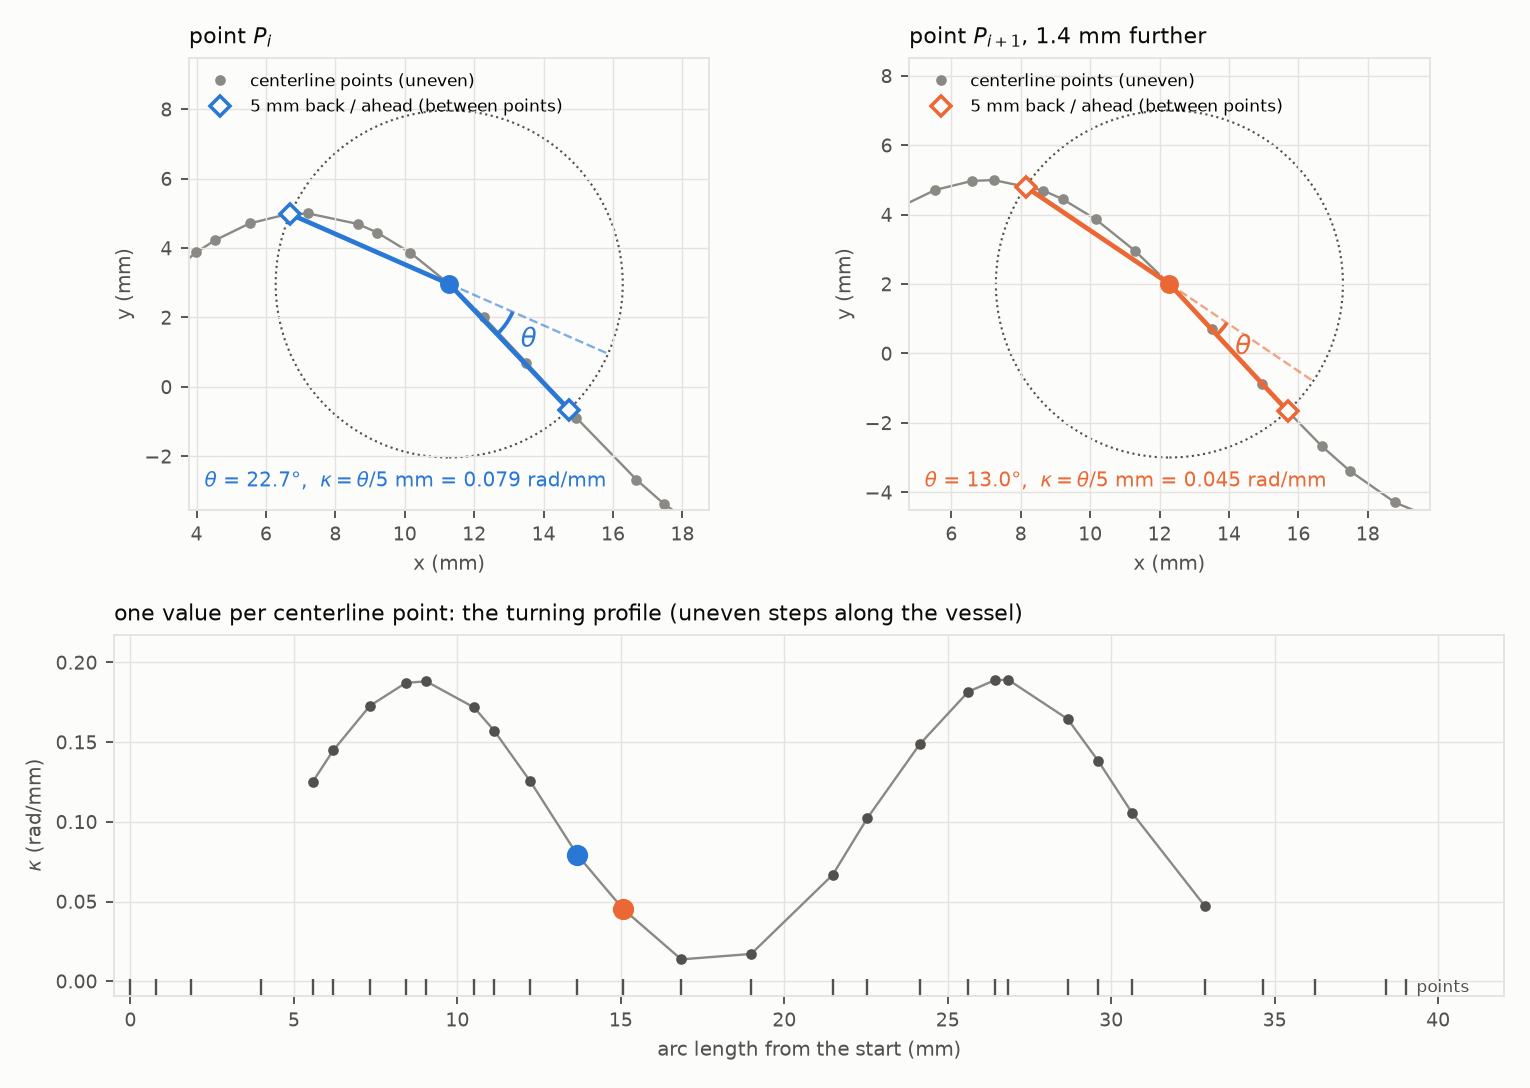
\includegraphics[width=1\textwidth]{week_figure/turning_sliding.png}
  \caption{Turning angle at every centerline point, on a made-up centerline with unevenly spaced
           points (grey). Top: at point $P_i$ (left) and at the next point $P_{i+1}$ (right), the
           chord ends (diamonds) lie 5\,mm away in a straight line (dotted circle), mostly between two
           points. The angle $\theta$ is the turn between the arriving chord, continued straight
           (dashed), and the leaving chord. Bottom: the resulting value at every point; the ticks show
           the uneven point spacing, and there is no value within 5\,mm of either end.}
  \label{fig:sliding}
\end{figure}

\textbf{Functional principal component analysis (FPCA).} The average profile is the same for everyone
and cannot separate people, so it is subtracted at each position:
\begin{equation}
  m_j = \frac{1}{n}\sum_i M_{ij}, \qquad D_{ij} = M_{ij} - m_j ,
\end{equation}
where $D_{ij} > 0$ means that person $i$ turns more than average at position $j$. The singular value
decomposition of $D$ gives the shapes $\varphi_1, \varphi_2, \dots$: $\varphi_1$ is the pattern along
which people differ most, $\varphi_2$ the next, and the shapes are perpendicular, so each describes
something the others do not. The share of the differences described by shape $k$ is
$\lambda_k / \sum_{k'}\lambda_{k'}$, where $\lambda_k$ is the variance of the scores along it. Person
$i$'s amount of shape $k$ is the score
\begin{equation}
  c_{ik} = \sum_{j} D_{ij}\,\varphi_{kj}, \qquad z_{ik} = c_{ik} / \mathrm{SD}_k ,
\end{equation}
where $\mathrm{SD}_k$ is the standard deviation of the scores over people. A positive score means the
person shows the shape, a negative score its opposite. The sign of a shape is arbitrary, so I fix it
such that $\sum_j \varphi_{kj} \geq 0$ and always read a shape as the average profile plus and minus
$2\,\mathrm{SD}_k \cdot \varphi_k$ (Figure~\ref{fig:shapes}). In the Medis profiles analysed so far,
$\varphi_1$ has the same sign along the whole segment, so its score is close to the person's mean
turning relative to the average, the main model's $T_5$.

\textbf{Number of shapes.} The number of shapes $K$ is fixed before the curvature profiles are linked
to the outcome, from three counts of the leading shapes: those stable over 200 bootstrap samples of
people (median $|\cos|$ between the bootstrap and the full-data shape $\geq 0.9$), those whose
variance exceeds the 95th percentile of 200 data sets with people permuted at each position (Horn's
parallel analysis), and the number that best predicts a held-out fifth of the profile in held-out
people (five-fold cross-validation). $K$ is the smallest of the three counts, capped at the Riley
maximum of 10 (pLAD) and 8 (mLAD).

\textbf{Model.} Each of the two models is the main model restricted to one segment. The main model
has nine rows per person, one per segment, and its person random intercept lets the rows of the
same person share a common level of risk. Here each person has a single row, so there is nothing to
share, and the random intercept is left out. The link, the SCORE2 base and the reading of the weights
are unchanged; only the curvature enters as $K$ shape scores instead of one mean:
\begin{equation}
  \mathrm{cloglog}(p_i) = a + g\,\mathrm{SCORE2}_i + \sum_{k=1}^{K} b_k\, z_{ik},
\end{equation}
where $p_i$ is the probability that person $i$ developed plaque in the segment and $e^{b_k}$ is the
hazard ratio per SD of shape $k$. A positive $b_k$ means that the shape as drawn (solid line) goes
with plaque, a negative $b_k$ that its opposite does. A likelihood-ratio test of
$\varphi_2, \dots, \varphi_K$ given $\varphi_1$ ($K - 1$ degrees of freedom) asks whether the shape of
the profile adds to the mean turning. The weights combine into one weight per position,
\begin{equation}
  \beta_j = \sum_{k=1}^{K} \frac{b_k}{\mathrm{SD}_k}\,\varphi_{kj},
\end{equation}
which I plot along the segment to show where more turning goes with more or less plaque. SCORE2 enters
in the same form as in the main model, which is still open (recalibrated or refitted).

\textbf{Limits.} The two tests are descriptive and not corrected for multiplicity. The shapes are
estimated in this cohort and would differ in another, so the scores are not comparable across
cohorts. The code (\texttt{CGPS\_data/turning\_profile\_shapes.py},
\texttt{segment\_k\_budget.py}) is exploratory; once the sliding-window profile is adopted, the
curvature section of the methods must be updated, as it still describes the turning angle at
vertices 5\,mm apart. The full worked explanation with made-up data is in \texttt{fpca\_explained.pdf}.

\begin{figure}[h]
  \centering
  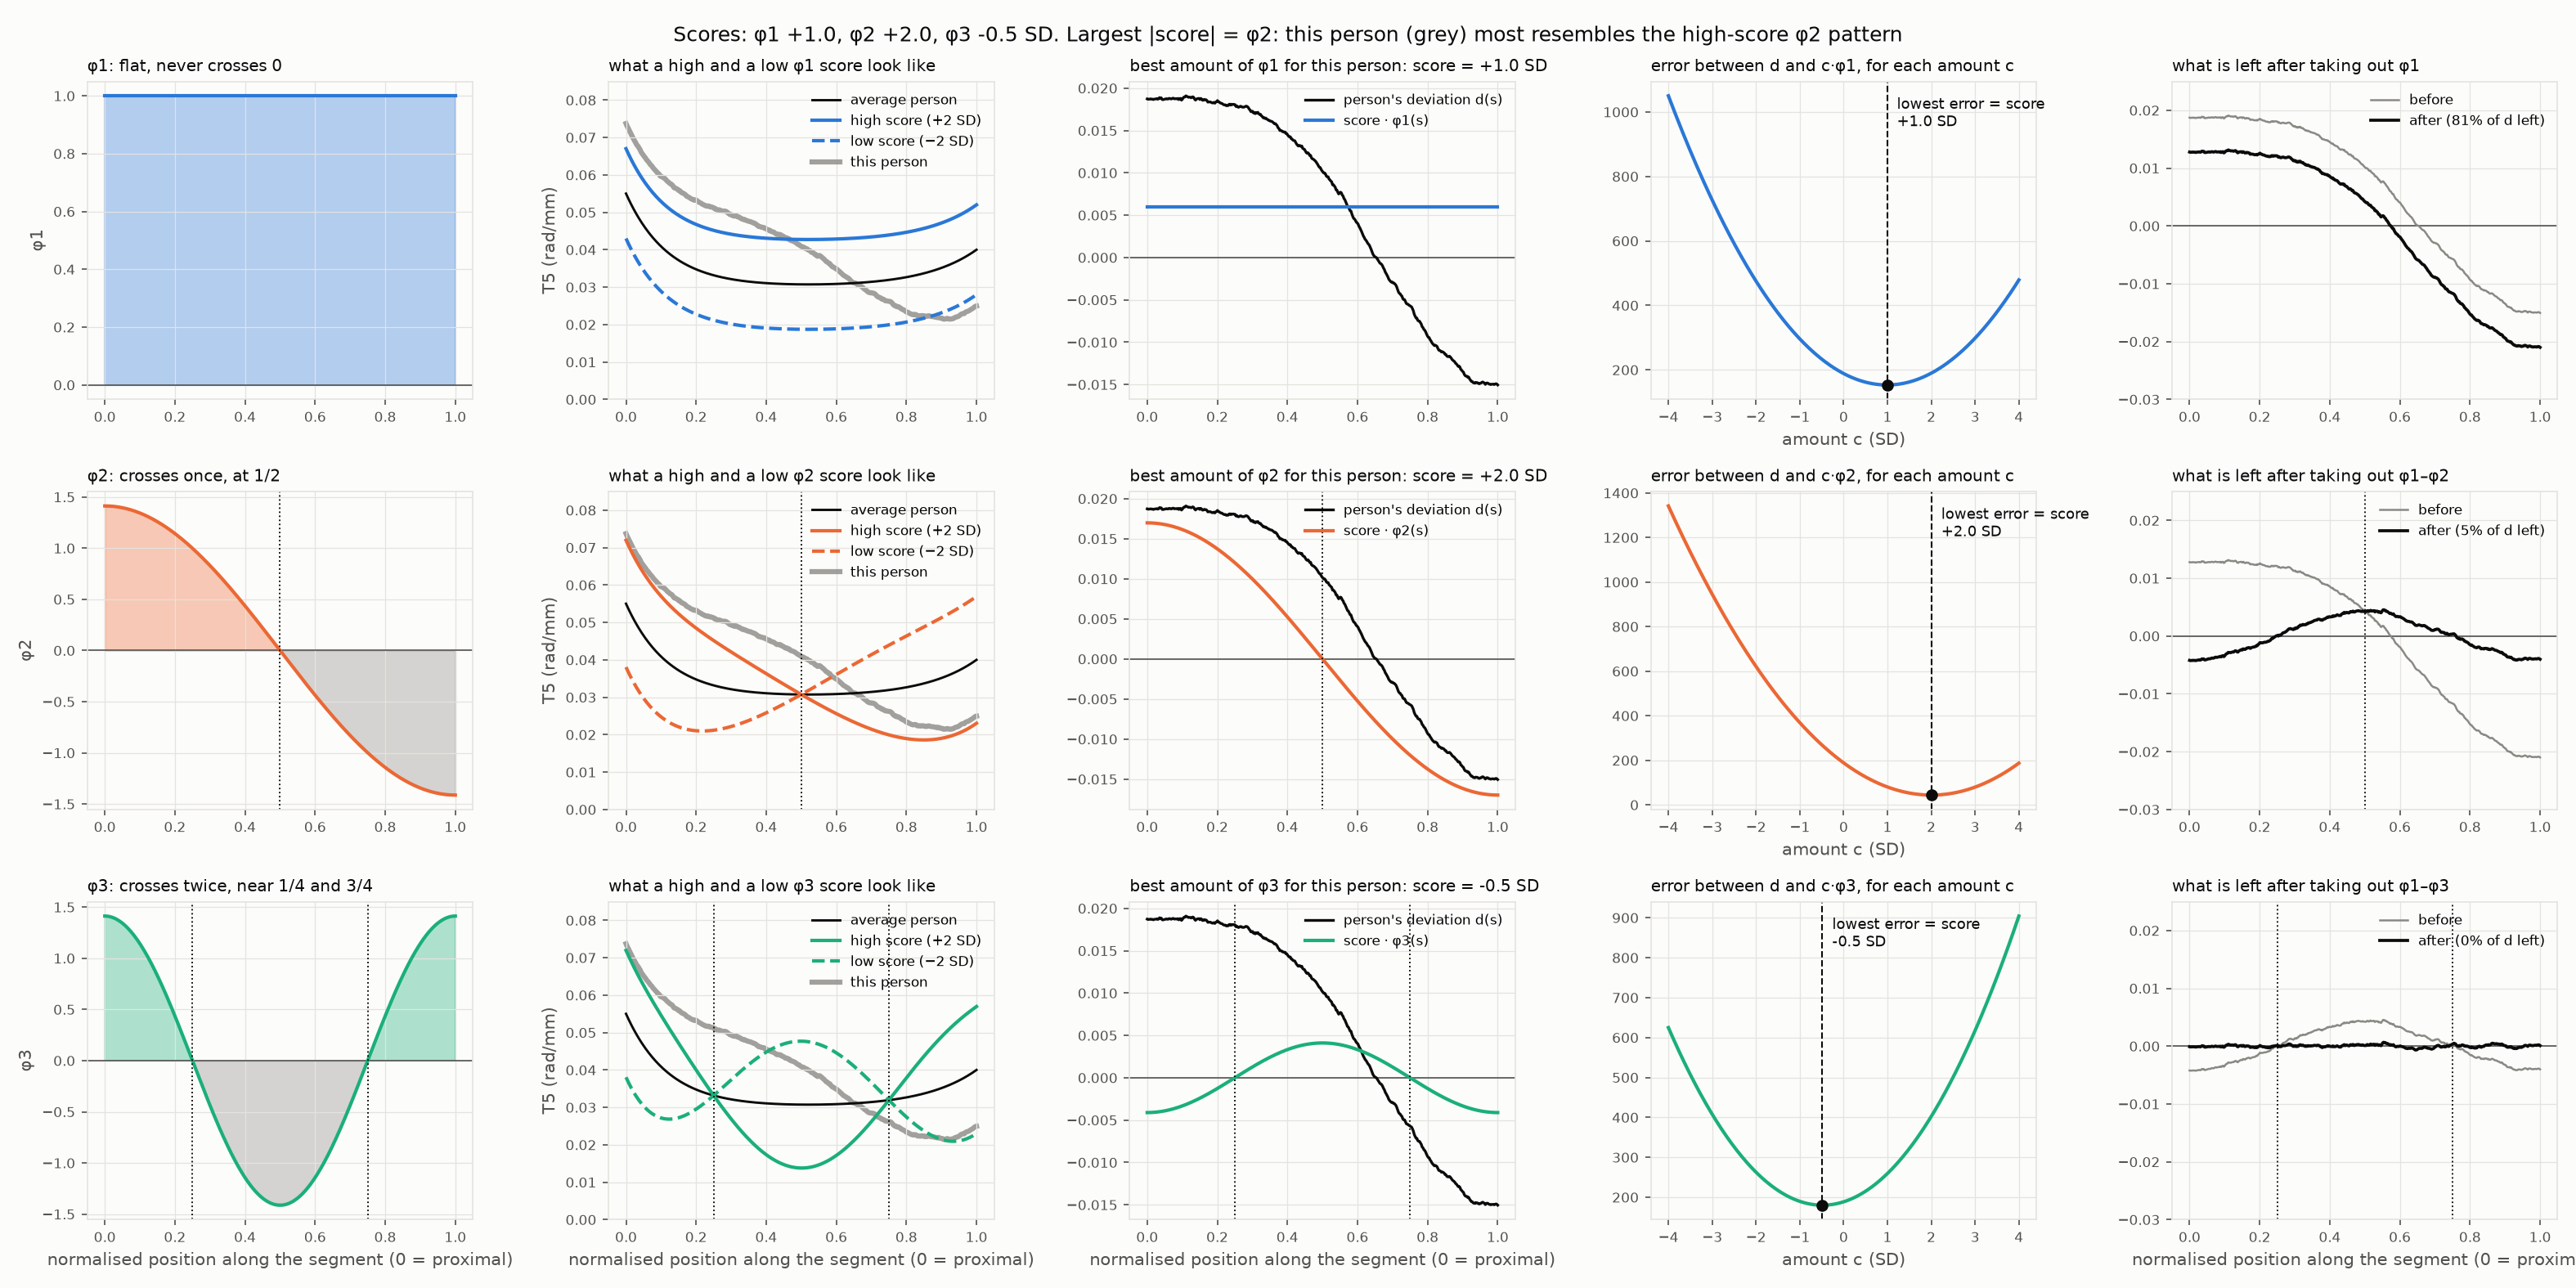
\includegraphics[width=1\textwidth]{week_figure/shape_scores_phi2_person.png}
  \caption{From profile to shape scores, with three idealised shapes and one made-up person. Rows are
           the shapes; columns show (1) the shape, (2) a high (solid) and low (dashed) scorer next
           to the average, (3) the person's deviation with score $\times\,\varphi_k$, (4) the error for
           each amount of the shape, whose minimum is the score, and (5) what remains after removing
           the shapes so far. The person resembles $\varphi_2$ most: more turning early, less late.}
  \label{fig:shapes}
\end{figure}
